% ---
% Capa
% ---
\imprimircapa
% ---

% ---
% Folha de rosto
% (o * indica que haverá a ficha bibliográfica)
% ---
\imprimirfolhaderosto*
% ---

% ---
% Inserir a ficha bibliografica
% ---
% http://ficha.bu.ufsc.br/
\begin{fichacatalografica}
	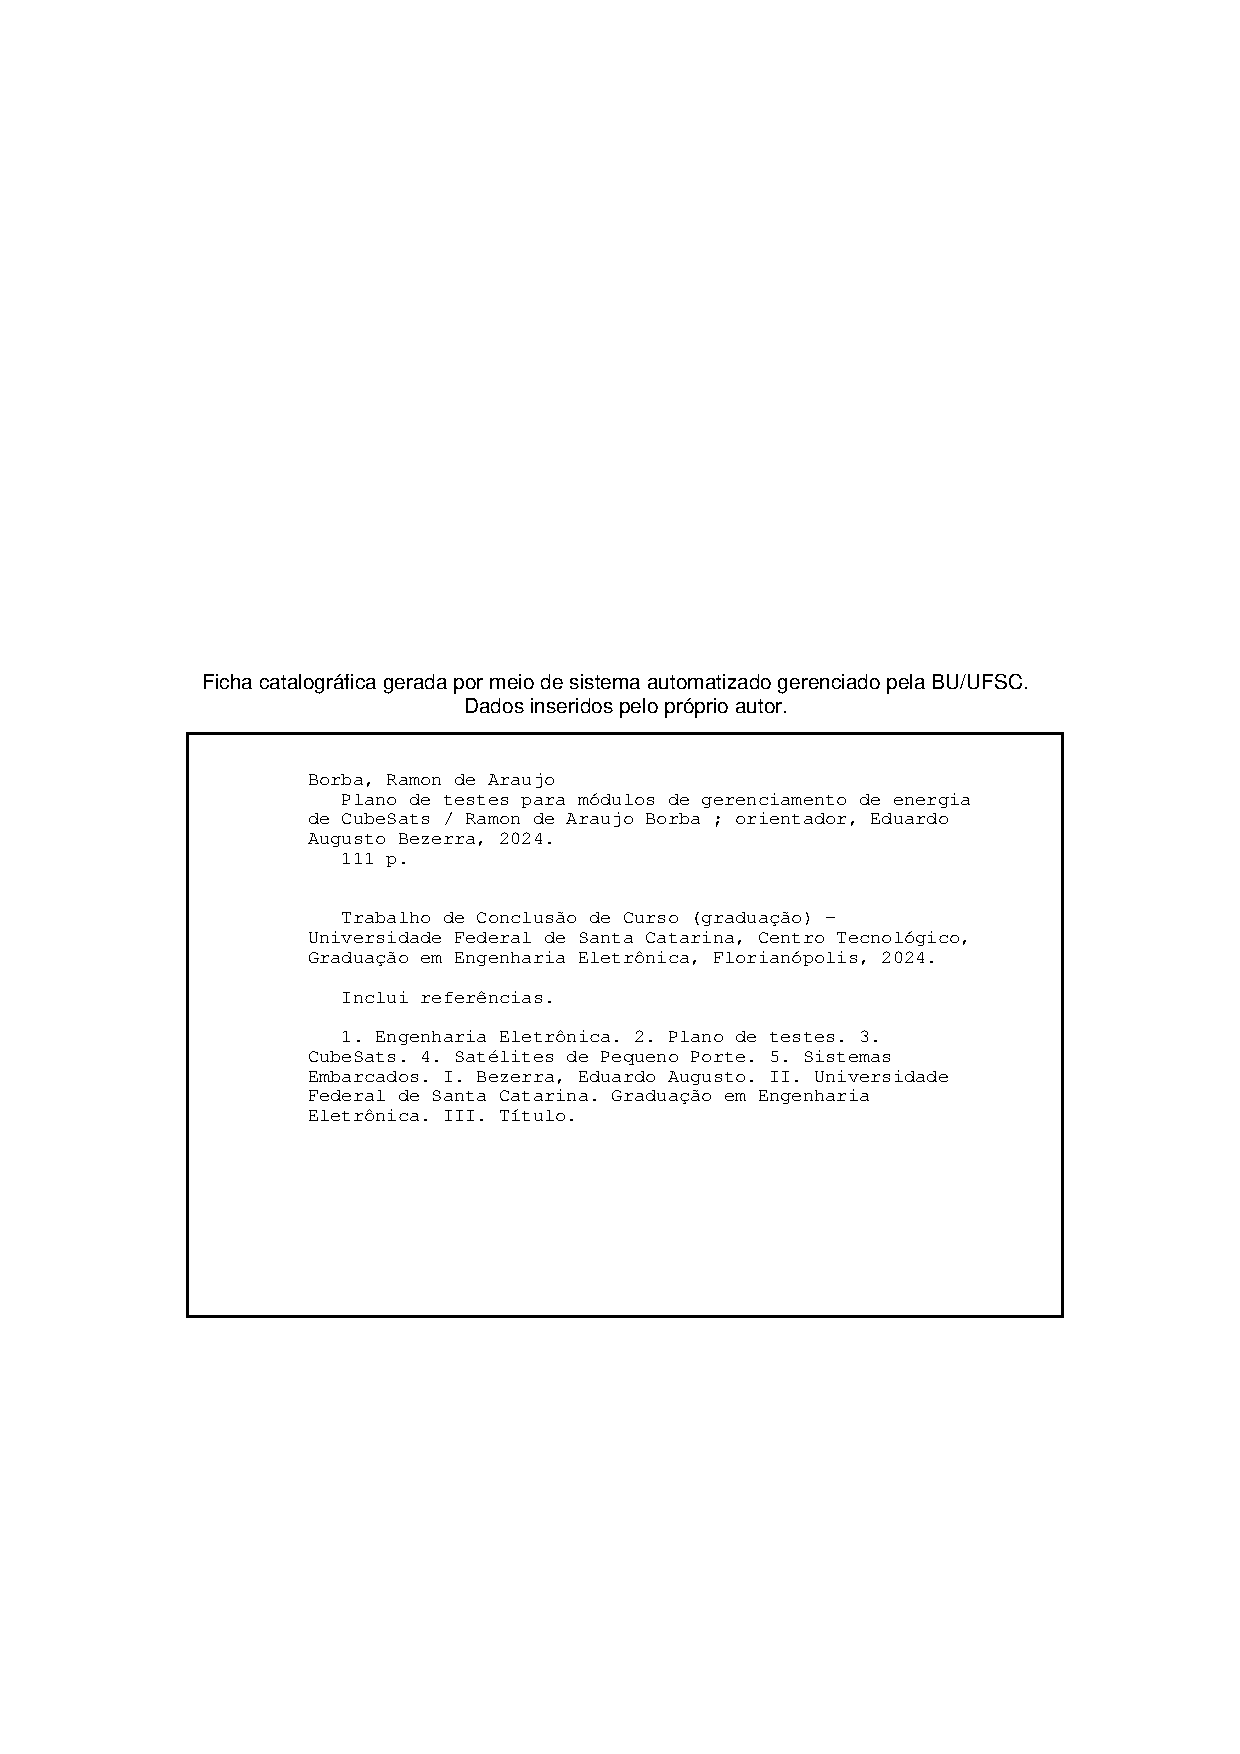
\includepdf{beforetext/Ficha_Catalografica.pdf}
\end{fichacatalografica}
% ---

% ---
% Inserir folha de aprovação
% ---
\begin{folhadeaprovacao}
	\OnehalfSpacing
	\centering
	\imprimirautor\\%
	\vspace*{10pt}		
	\textbf{\imprimirtitulo}%
	\ifnotempty{\imprimirsubtitulo}{:~\imprimirsubtitulo}\\%
	%		\vspace*{31.5pt}%3\baselineskip
	\vspace*{\baselineskip}
	%\begin{minipage}{\textwidth}
	% ~do~\imprimirprograma~do~\imprimircentro~da~\imprimirinstituicao~para~a~obtenção~do~título~de~\imprimirformacao.
	Este~\imprimirtipotrabalho~foi julgado adequado para obtenção do Título de “\imprimirformacao” e aprovado em sua forma final pelo~\imprimirprograma. \\
		\vspace*{\baselineskip}
	\imprimirlocal, \imprimirdata. \\
	\vspace*{\baselineskip}
	\assinatura{\OnehalfSpacing\imprimircoordenador \\ \imprimircoordenadorRotulo~do Curso}
	\vspace*{\baselineskip}
	\textbf{Banca Examinadora:} \\
	\vspace*{\baselineskip}
	\assinatura{\OnehalfSpacing\imprimirorientador \\ \imprimirorientadorRotulo}
	%\end{minipage}%
	\vspace*{\baselineskip}
	\assinatura{Kleber Gouveia, Msc.\\
	Avaliador \\
	Universidade Federal de Santa Catarina}

	\vspace*{\baselineskip}
	\assinatura{Gabriel Mariano Marcelino, Msc.\\
	Avaliador \\
	Universidade Federal de Santa Catarina}


	\vspace*{\baselineskip}
	\assinatura{João Cláudio Elsen Barcellos, Eng.\\
	Avaliador \\
	Universidade Federal de Santa Catarina}

\end{folhadeaprovacao}
% ---

% ---
% Dedicatória
% ---
\begin{dedicatoria}
	\vspace*{\fill}
	\noindent
	\begin{adjustwidth*}{}{5.5cm}     
		Este trabalho é dedicado aos meus queridos pais e a minha família por todo o apoio nesta caminhada.
	\end{adjustwidth*}
\end{dedicatoria}
% ---

% ---
% Agradecimentos
% ---
\begin{agradecimentos}
	Agradeço primeiramente aos meus pais, Valeria e Regis, sempre estarem ao meu lado e pelo amor imensurável.
	
	Agradeço à minha família por me apoiarem incondicionalmente durante toda esta jornada.
	
	Agradeço à minha companheira Thaysi por todo amor, carinho e compreensão.

	Agradeço ao meu orientador prof. Eduardo Bezerra pela confiança e pelas oportunidades proporcionadas.
	
	Agradeço ao meu colega e amigo João Cláudio, pelo apoio, discussões e ideias compartilhadas.
	
	Agradeço aos meus colegas de laboratório e graduação pelo companheirismo, união e por tornarem os dias difíceis mais leves.
\end{agradecimentos}
% ---

% ---
% Epígrafe
% ---
\begin{epigrafe}
	\vspace*{\fill}
	\begin{flushright}
		% \textit{``Texto da Epígrafe.\\
		% 	Citação relativa ao tema do trabalho.\\
		% 	É opcional. A epígrafe pode também aparecer\\
		% 	na abertura de cada seção ou capítulo.\\
		% 	Deve ser elaborada de acordo com a NBR 10520.''\\
		% 	(Autor da epígrafe, ano)}
	\end{flushright}
\end{epigrafe}
% ---

% ---
% RESUMOS
% ---

% resumo em português
\setlength{\absparsep}{18pt} % ajusta o espaçamento dos parágrafos do resumo
\begin{resumo}
	\SingleSpacing
	Os CubeSats, apesar de estarem se popularizando rapidamente, ainda apresentam taxas de falha significativas, especialmente em missões universitárias. Em grande quantidade dos CubeSats lançados, o módulo de gerenciamento de energia é acusado como o principal causador de falhas. Isso se dá principalmente por uma falta de atenção aos procedimentos de verificação e testes destes módulos. Em missões mais recentes, com o intuito de mitigar as altas taxas de falha, normas mais rigorosas, de instituições como ECSS, vem sendo adotadas, porém ainda não aplicadas a nível de modulo. Com isto em mente, foi proposta a elaboração de um documento contendo diretrizes e orientações acerca da preparação de planos de teste para módulos de gerenciamento de energia de CubeSats, baseado em normas da ECSS, de forma que possa ser aplicado à diferentes topologias e arquiteturas. Para este objetivo, foi conduzida uma revisão de diferentes arquiteturas e topologias destes módulos, bem como das campanhas de testes aplicadas. Também, uma análise das normas relacionadas à testes e seu principais conceitos foi conduzida, avaliando as principais considerações necessárias em relação à aplicação destas normas a um módulo de CubeSat. A partir destas análises, o documento proposto foi elaborado e nomeado \textit{EPS Test Plan Guidelines}. Por fim, como demonstração destes conceitos, um plano de testes para o módulo de gerenciamento de energia EPS 2.0, desenvolvido pelo SpaceLab, foi proposto.
	
	\textbf{Palavras-chave}: Plano de Testes. CubeSat. Satélites de Pequeno Porte. Sistemas Embarcados.
\end{resumo}

% resumo em inglês
\begin{resumo}[Abstract]
	\SingleSpacing
	\begin{otherlanguage*}{english}
		CubeSats, even though quickly rising in popularity, still present significant failure rates, specially in university missions. In a great portion of launched CubeSats, the electrical power system module is accused as the main cause of failure. This is mainly caused by a lack of attention to the verification and testing processes of these modules. In more recent missions, with the intent of mitigating the high failure rates, more rigorous standards, from institutions such as ECSS, are being adoptes, but still not applied at module level. With that in mind, it was proposed the elaboration of a document containing guidelines and orientations regarding the preparation of test plans for CubeSat electrical power system modules, based on the ECSS standards, intended to be applicable to different topologies and architectures. For this purpose, a review was conducted of different architectures and topologies of these modules, as well as the applied test campaigns. Also, an analysis was conducted of the relevant standards related to testing and it's main concepts, evaluating the main considerations needed regarding the application of these standards to a CubeSat module. From those analysis, the proposed document was elaborated and named EPS Test Plan Guidelines. And last, as a demonstration of these concepts, a test plan for the EPS 2.0 electrical power system module, developed at SpaceLab, was proposed.
		
		\textbf{Keywords}: Test Plan. CubeSat. Small Satellites. Embedded Systems.
	\end{otherlanguage*}
\end{resumo}

%% resumo em francês 
%\begin{resumo}[Résumé]
% \begin{otherlanguage*}{french}
%    Il s'agit d'un résumé en français.
% 
%   \textbf{Mots-clés}: latex. abntex. publication de textes.
% \end{otherlanguage*}
%\end{resumo}
%
%% resumo em espanhol
%\begin{resumo}[Resumen]
% \begin{otherlanguage*}{spanish}
%   Este es el resumen en español.
%  
%   \textbf{Palabras clave}: latex. abntex. publicación de textos.
% \end{otherlanguage*}
%\end{resumo}
%% ---

{%hidelinks
	\hypersetup{hidelinks}
	% ---
	% inserir lista de ilustrações
	% ---
	\pdfbookmark[0]{\listfigurename}{lof}
	\listoffigures*
	\cleardoublepage
	% ---
	
	% ---
	% inserir lista de quadros
	% ---
	% \pdfbookmark[0]{\listofquadrosname}{loq}
	% \listofquadros*
	% \cleardoublepage
	% ---
	
	% ---
	% inserir lista de tabelas
	% ---
	\pdfbookmark[0]{\listtablename}{lot}
	\listoftables*
	\cleardoublepage
	% ---
	
	% ---
	% inserir lista de abreviaturas e siglas (devem ser declarados no preambulo)
	% ---
	\imprimirlistadesiglas
	% ---
	
	% ---
	% inserir lista de símbolos (devem ser declarados no preambulo)
	% ---
	% \imprimirlistadesimbolos
	% ---
	
	% ---
	% inserir o sumario
	% ---
	\pdfbookmark[0]{\contentsname}{toc}
	\tableofcontents*
	\cleardoublepage
	
}%hidelinks
% ---